\chapter{Concetti generici di una web app}
\section{Che cos'è una web app}
Una web app è un software applicativo eseguito su un server web, accessibile e utilizzabile da un utente tramite un browser.\cite{webApp1}
Un'applicazione web è costituita da:
\begin{itemize}
    \item Back-end: si occupa, lato server, di tutta la logica dell'applicazione, della gestione dei dati e della comunicazione con il database.
    \item Front-end: si occupa, lato client, della presentazione delle informazioni all'utente garantendo l'interazione tra utente e applicazione web.
\end{itemize}
\section{Architettura di una web app}
Una web app possiede la seguente architettura (Figura \ref{fig:funzionamento-web-app}):
\begin{enumerate}
    \item L'utente, tramite un'interfaccia dell'applicazione, invia una richiesta al server;
    \item Il client inoltra la richiesta dell'utente al server;
    \item Il server esegue l'operazione richiesta, generando i risultati dei dati richiesti;
    \item Il server invia i risultati al client, il quale si occuperà di visualizzarli all'utente.
\end{enumerate}
\begin{figure}[h]
    \centering
    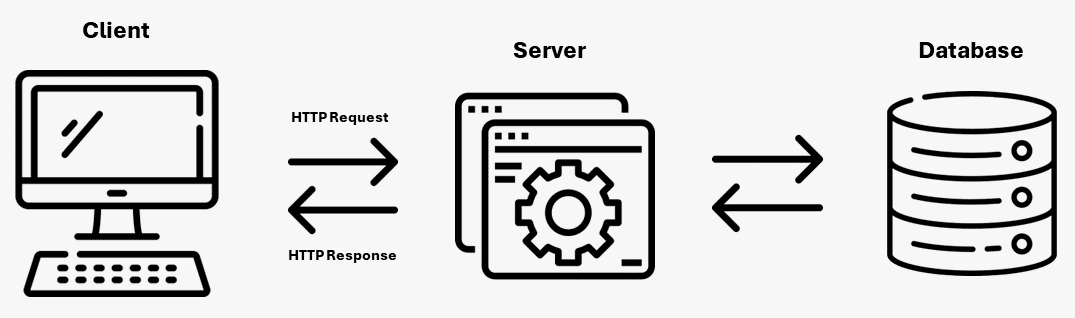
\includegraphics[width=0.9\textwidth]{images/funzionamentoWebApp.png}
    \caption{Funzionamento di un'applicazione web}
    \label{fig:funzionamento-web-app}
\end{figure}